\documentclass[xetex,mathserif,serif]{beamer}
\usepackage{polyglossia}
\setdefaultlanguage[babelshorthands=true]{russian}
\usepackage{minted}
\usepackage{tabu}

\useoutertheme{infolines}

\usepackage{fontspec}
\setmainfont{FreeSans}
\newfontfamily{\russianfonttt}{FreeSans}

\usepackage{textpos}
\setlength{\TPHorizModule}{1cm}
\setlength{\TPVertModule}{1cm}

\setbeamertemplate{blocks}[rounded][shadow=false]

\setbeamercolor*{block title alerted}{fg=red!50!black,bg=red!20}
\setbeamercolor*{block body alerted}{fg=black,bg=red!10}

\tabulinesep=1.2mm

\title{Занятие 6: Планирование}
\author[Юрий Литвинов]{Юрий Литвинов\\\small{\textcolor{gray}{yurii.litvinov@gmail.com}}}
\date{18.10.2017}

\newcommand{\attribution}[1] {
	\begin{flushright}\begin{scriptsize}\textcolor{gray}{\textcopyright\; #1}\end{scriptsize}\end{flushright}
}

\begin{document}

	\frame{\titlepage}

	\section{Задание на пару}

	\begin{frame}
		\frametitle{Диаграмма Гантта}
		\begin{center}
			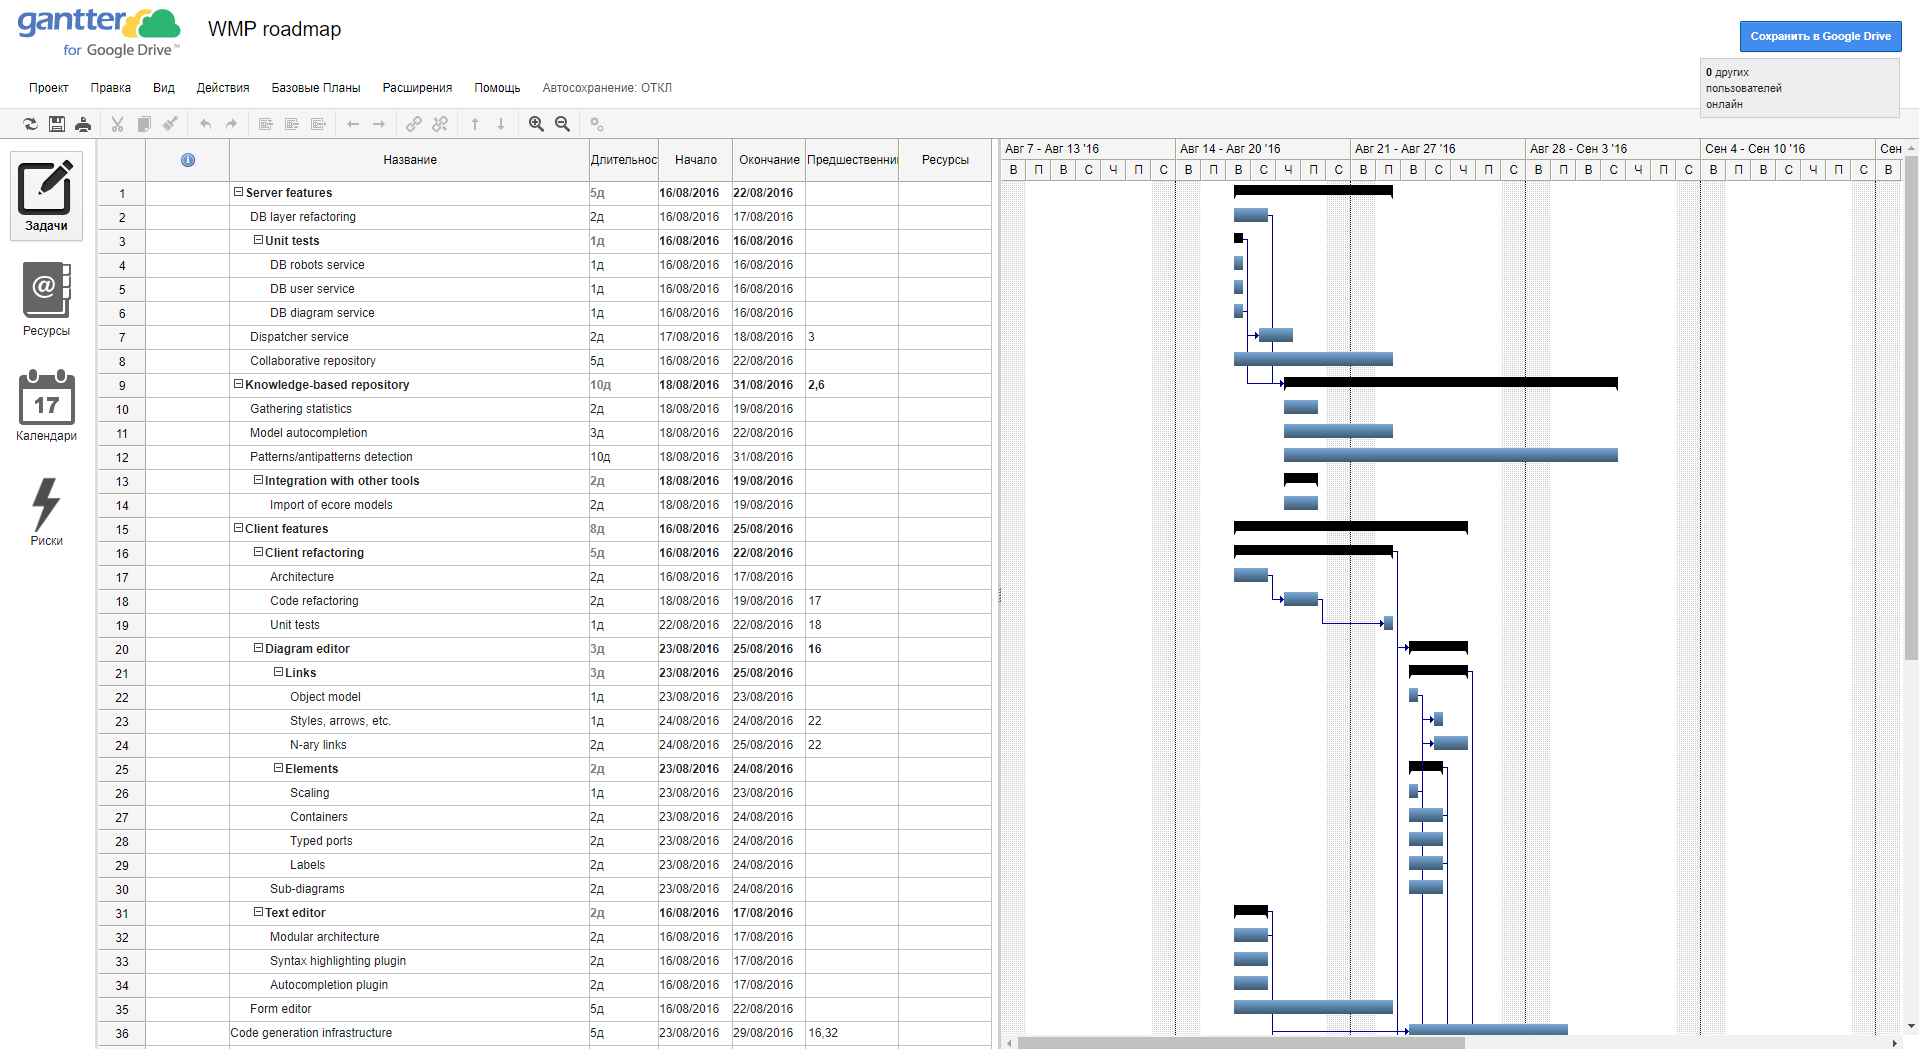
\includegraphics[width=\textwidth]{gantter.png}
		\end{center}
	\end{frame}

	\begin{frame}
		\frametitle{Задание на пару}
		\begin{itemize}
			\item Нарисовать диаграмму Гантта для своего проекта
			\begin{itemize}
				\item Использовать декомпозицию и оценки с предыдущей пары
				\item Получить календарный график работ
				\item Пока без привязки к ресурсам
			\end{itemize}
			\item Доделать дома и выложить на вики проекта
		\end{itemize}
	\end{frame}

\end{document}
